%!TEX program = xelatex
\documentclass[dvipsnames, svgnames,a4paper,11pt]{article}
% ----------------------------------------------------- 
%	加边框的命令
%	参考:https://tex.stackexchange.com/questions/531559/how-to-add-the-page-border-for-first-two-pages-in-latex
\usepackage{tikz}
\usetikzlibrary{calc}
\usepackage{eso-pic}
\AddToShipoutPictureBG{%
\begin{tikzpicture}[overlay,remember picture]
\draw[line width=0.6pt] % 边框粗细
    ($ (current page.north west) + (0.6cm,-0.6cm) $)
    rectangle
    ($ (current page.south east) + (-0.6cm,0.6cm) $); % 边框位置
\end{tikzpicture}}


\usepackage{xcolor}
\definecolor{c1}{HTML}{086173} % 目录颜色 原版为2752C9 紫灰色535AAA 蓝紫色0B0DB7 深蓝色070F94 湖绿色219394 松石灰绿086173
\definecolor{c2}{HTML}{E20129} % 引用颜色 原版\definecolor{c2}{RGB}{190,20,83} 橙色F24729

\usepackage{ctex}
\usepackage[top=28mm,bottom=28mm,left=15mm,right=15mm]{geometry}
\usepackage{hyperref} 
\hypersetup{
	colorlinks,
	linktoc = section, % 超链接位置,选项有section, page, all
	linkcolor = c1, % linkcolor 目录颜色
	citecolor = c1  % citecolor 引用颜色
}
\usepackage{amsmath,enumerate,multirow,float}
\usepackage{tabularx}
\usepackage{tabu}
\usepackage{subfig}
\usepackage{fancyhdr}
\usepackage{graphicx}
\usepackage{wrapfig}  
\usepackage{physics}
\usepackage{appendix}
\usepackage{amsfonts}

%
\usepackage{tcolorbox}
\tcbuselibrary{skins,breakable}
\newtcolorbox{tbox}[2][]{
    colframe=black!70!,
    breakable,
    enhanced,
	boxrule =0.5pt,
    title = {#2},
    fonttitle = \large\kaishu\bfseries,
	drop fuzzy shadow,
    #1
}
\newtcolorbox[auto counter,number within=section]{question}[1][]{
  top=2pt,bottom=2pt,arc=1mm,
  boxrule=0.5pt,
%   frame hidden,
  breakable,
  enhanced, %跨页后不会显示下边框
  coltitle=c1!80!gray,
  colframe=c1,
  colback=c1!3!white,
  drop fuzzy shadow,
  title={思考题~\thetcbcounter:\quad},
  fonttitle=\bfseries,
  attach title to upper,
  #1
}

% ---------------------------------------------------------------------
%	利用cleveref改变引用格式,\cref是引用命令
\usepackage{cleveref}
\crefformat{figure}{#2{\textcolor{c2}{Figure #1}}#3} % 图片的引用格式
\crefformat{equation}{#2{(\textcolor{c2}{#1})}#3} % 公式的引用格式
\crefformat{table}{#2{\textcolor{c2}{Table #1}}#3} % 表格的引用格式


% ---------------------------------------------------------------------
%	页眉页脚设置
\fancypagestyle{plain}{\pagestyle{fancy}}
\pagestyle{fancy}
\lhead{\kaishu 中山大学物理与天文学院电子技术实验\uppercase\expandafter{\romannumeral1}} % 左边页眉,学院 + 课程
\rhead{\kaishu 实验报告By黄罗琳} % 右边页眉,实验报告标题
\cfoot{\thepage} % 页脚,中间添加页码


% ---------------------------------------------------------------------
%	对目录、章节标题的设置
\renewcommand{\contentsname}{\centerline{\huge 目录}}
\usepackage{titlesec}
\usepackage{titletoc}
% \titleformat{章节}[形状]{格式}{标题序号}{序号与标题间距}{标题前命令}[标题后命令]
\titleformat{\section}{\centering\LARGE\songti}{}{1em}{}

% ---------------------------------------------------------------------
%   listing代码环境设置
\usepackage{listings}
\lstloadlanguages{python}
\lstdefinestyle{pythonstyle}{
backgroundcolor=\color{gray!5},
language=python,
frameround=tftt,
frame=shadowbox, 
keepspaces=true,
breaklines,
columns=spaceflexible,                   
basicstyle=\ttfamily\small, % 基本文本设置,字体为teletype,大小为scriptsize
keywordstyle=[1]\color{c1}\bfseries, 
keywordstyle=[2]\color{Red!70!black},   
stringstyle=\color{Purple},       
showstringspaces=false,
commentstyle=\ttfamily\scriptsize\color{green!40!black},%注释文本设置,字体为sf,大小为smaller
tabsize=2,
morekeywords={as},
morekeywords=[2]{np, plt, sp},
numbers=left, % 代码行数
numberstyle=\it\tiny\color{gray}, % 代码行数的数字字体设置
stepnumber=1,
rulesepcolor=\color{gray!30!white}
}




% ---------------------------------------------------------------------
%	其他设置
\def\degree{${}^{\circ}$} % 角度
\graphicspath{{./images/}} % 插入图片的相对路径
\allowdisplaybreaks[4]  %允许公式跨页 
\usepackage{lipsum}
\usepackage{adjustbox}
%\usepackage{mathrsfs} % 字体
%\captionsetup[figure]{name=Figure} % 图片形式
%\captionsetup[table]{name=Table} % 表格形式
\begin{document}
	
	% 实验报告封面	
	% 顶栏
	\begin{table}
		\renewcommand\arraystretch{1.7}
		\begin{tabularx}{\textwidth}{
				|X|X|X|X
				|X|X|X|X|}
			\hline
			\multicolumn{2}{|c|}{预习报告}&\multicolumn{2}{|c|}{实验记录}&\multicolumn{2}{|c|}{分析讨论}&\multicolumn{2}{|c|}{总成绩}\\
			\hline
			\LARGE25 & & \LARGE25 & & \LARGE30 & & \LARGE80 & \\
			\hline
		\end{tabularx}
	\end{table}
	% ---
	
	% 信息栏
		\begin{table}
		\renewcommand\arraystretch{1.7}
		\begin{tabularx}{\textwidth}{|X|X|X|X|}
			\hline
			年级、专业: & 2022级 物理学 &组号: & \\
			\hline
			姓名: &  黄罗琳,王显  & 学号: &22344001 22344002   \\
			\hline
			实验时间: & 2024/3/20 & 教师签名: & \\
			\hline
		\end{tabularx}
	\end{table}
	% ---
	
	% 大标题
	\begin{center}
	\LARGE ET4 \quad 戴维南定理和诺顿定理
	\end{center}
	% ---
	
	% 注意事项
	
	% 基本
	\textbf{【实验报告注意事项】}
	\begin{enumerate}
		\item 实验报告由三部分组成:
		\begin{enumerate}
			\item 预习报告:课前认真研读实验讲义,弄清实验原理;实验所需的仪器设备、用具及其使用、完成课前预习思考题;了解实验需要测量的物理量,并根据要求提前准备实验记录表格(可以参考实验报告模板,可以打印)。\textcolor{red}{\textbf{(20分)}}
			\item 实验记录:认真、客观记录实验条件、实验过程中的现象以及数据。实验记录请用珠笔或者钢笔书写并签名(\textcolor{red}{\textbf{用铅笔记录的被认为无效}})。\textcolor{red}{\textbf{保持原始记录,包括写错删除部分,如因误记需要修改记录,必须按规范修改。}}(不得输入电脑打印,但可扫描手记后打印扫描件);离开前请实验教师检查记录并签名。\textcolor{red}{\textbf{(30分)}}
			\item 数据处理及分析讨论:处理实验原始数据(学习仪器使用类型的实验除外),对数据的可靠性和合理性进行分析;按规范呈现数据和结果(图、表),包括数据、图表按顺序编号及其引用;分析物理现象(含回答实验思考题,写出问题思考过程,必要时按规范引用数据);最后得出结论。\textcolor{red}{\textbf{(30分)}}
		\end{enumerate}
		\textbf{实验报告就是将预习报告、实验记录、和数据处理与分析合起来,加上本页封面。\textcolor{red}{(80分)}}
		\item 每次完成实验后的一周内交\textbf{实验报告}(特殊情况不能超过两周)。
		\item \textbf{其它注意事项}:
		\begin{enumerate}
			\item 请认真查看并理解实验讲义第一章内容;
			\item 注意实验器材的合理使用;
			\item 使用结束使用各种仪器之后需要将其放回原位。
		\end{enumerate}
	\end{enumerate}
	

	% 目录
	\clearpage
	\tableofcontents
	\clearpage
	% ---
	
	
	
	% 预习报告	
	
	% 小标题
	\setcounter{section}{0}
\section{ET4戴维南定理和诺顿定理 \quad\heiti 预习报告}
	% ---
	
	% 实验目的
	\subsection{实验目的}
	\begin{enumerate}
		\item 加深对戴维南定理和诺顿定理的理解。
	\item 学习戴维南等效参数的各种测量方法。
	\item 理解等效置换的概念。
	\item 学习直流稳压电源、万用表、直流电流表和电压表的正确使用方法。
	\end{enumerate}
	% ---
	
	% 仪器用具
	\subsection{仪器用具}
	\begin{table}[htbp]
		\centering
		\renewcommand\arraystretch{1.6}
		% \setlength{\tabcolsep}{10mm}
		\begin{tabular}{|p{0.05\textwidth}|p{0.20\textwidth}|p{0.05\textwidth}|p{0.5\textwidth}|}
			\hline
			编号& 仪器用具名称 & 数量 &  主要参数(型号,测量范围,测量精度等) \\
			\hline
			1& 电路原理箱或板 & 1 &  \\
			\hline
			2& 稳压源 & 1 &  \\
			\hline
			3& 直流电流源 & 1 &  \\
			\hline
			4& 直流电流表 & 3 &  \\
			\hline
			5& 直流电压表 & 2 &  \\
			\hline
			6& 电流表专用线 & 3 &  \\
			\hline
			7& 2号实验导线 & n &  \\
			\hline
			8& 其它 & -- &  \\
			\hline
		\end{tabular}
	\end{table}
	% ---
	
	% 原理概述
	\subsection{原理概述}
	\begin{enumerate}
	\item \textbf{戴维南定理}指出:对于一个含有独立电源、线性电阻和受控源的一端口,可以用一个电压源和电阻的串联组合来等效置换。其中,该电压源的激励电压等于端口的开路电压,电阻等于将端口内全部独立电源置零后的输入电阻。
	\item \textbf{诺顿定理}是戴维南定理的对偶形式。它指出:对于一个含有独立电源、线性电阻和受控源的一端口,可以用一个电流源和电阻的并联组合来等效置换。电流源的激励电流等于端口的短路电流,电阻等于将端口中全部独立源置零后的输入电阻。
	\item \textbf{戴维南-诺顿定理的等效电路}是对外部特性而言的。换句话说,无论网络内部是时变的还是定常的,只要网络内部除了独立电源外都是线性元件,上述等效电路都是正确的。测量戴维南等效电路参数的方法:对于开路电压 $U_{oc}$ 的测量,可以直接使用电压表测量,也可以采用补偿法测量;而对于戴维南等效电阻 $R_{eq}$ 的获取,可采用如下方法:当网络含有源时,可以使用开路电压法或者短路电流法,但对于不允许直接短路外部电路的网络(例如,可能因短路电流过大而损坏网络内部器件的情况),不能采用短路电流法;当网络不含源时,可以使用伏安法、半流法、半压法、直接测量法等方法。
\end{enumerate}
\begin{figure}[H]
	\centering
	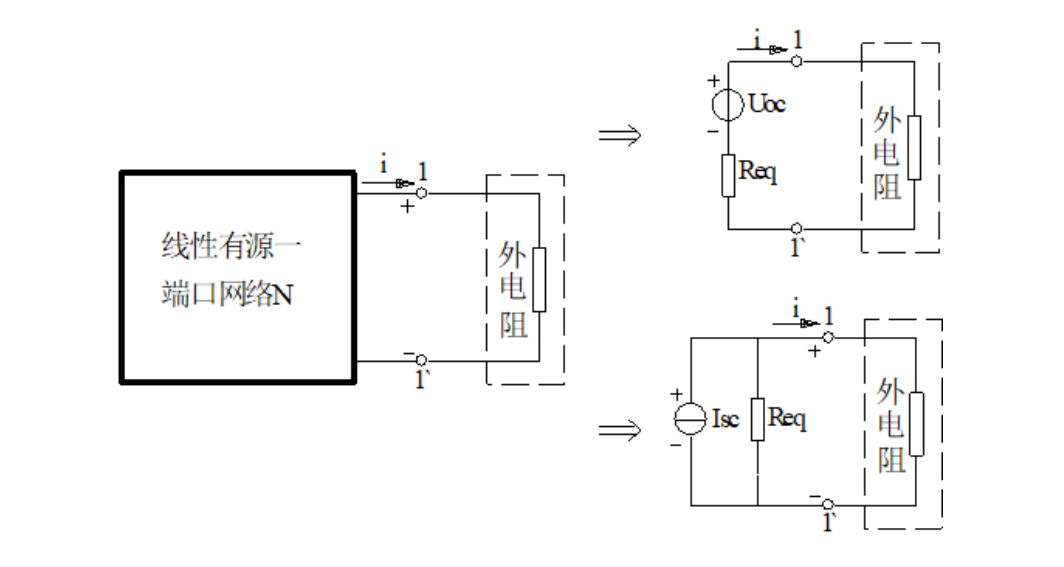
\includegraphics[width=0.4\linewidth]{images/一种端口}
	\caption{一种端口网络的等效置换}
	\label{fig:}
\end{figure}
	% ---
	
	
	
	% 实验前思考题
	\subsection{实验预习题}
	
\begin{question}
	用开路电压、短路电流法测量等效电阻时,开路电压、短路电流是否可以同时进行测量,为什么?
\end{question}

在使用开路电压和短路电流法测量电路的等效电阻时,实际操作中开路电压和短路电流是不能同时进行测量的。原因在于这两种测量方式的条件和对电路的影响完全不同。

\textbf{开路电压测量}:在进行开路电压的测量时,测量对象的两端不接任何外部负载,即电路是开路状态。这种测量方式的目的是测定在无负载条件下电源的电压,即电源的最大电动势。在这种状态下,电路中的电流为零,因此不会有电流通过被测电源或电路,可以获得一个准确的开路电压值。

\textbf{短路电流测量}:而在进行短路电流的测量时,测量对象的两端被直接短路,通过一个极低的电阻(接近于零),目的是测量在这种极端条件下通过电路的电流大小。这种状态下电路的电阻最小,电流达到最大值。这样做可以确定电源或电路在最大负载条件下的输出电流能力。

由于开路状态下电路的电流为零,而短路状态下电流达到最大,这两种状态下的电路条件截然不同,因此不能同时进行测量。同时,若尝试同时进行这两种测量,可能会导致测量结果不准确,甚至损坏测量设备或被测电路。通常,在实际应用中,先后分别进行这两种测量,然后通过欧姆定律(V=IR)计算出等效电阻值,即使用开路电压除以短路电流的方法得到等效电阻值:$ R_{\text{等效}} = \dfrac{V_{\text{开路}}}{I_{\text{短路}}} $。
	
	
	% 实验记录	
	\clearpage
	
	% 顶栏
	\begin{table}
		\renewcommand\arraystretch{1.7}
		\centering
		\begin{tabularx}{\textwidth}{|X|X|X|X|}
			\hline
			专业: & 物理学 & 年级: & 2022级 \\
			\hline
			姓名: & 黄罗琳,王显& 学号: &22344001,22344002 \\
			\hline
			室温: &  25℃& 实验地点: & A522 \\
			\hline
			学生签名:&  & 评分: &\\
			\hline
			实验时间:& 2024/3/20 & 教师签名:&\\
			\hline
		\end{tabularx}
	\end{table}
	% ---
	
	% 小标题
	\section{ETX 实验名称×××  \quad\heiti 实验记录}
	% ---
	
	% 实验过程记录
	\subsection{实验内容、步骤与结果}
	
	%
	\subsubsection{测量开路电压,短路电流} 
	设定Usn=12V
	\begin{enumerate}
		\item
		直接测量法
		 \begin{figure}[H]
			\centering
			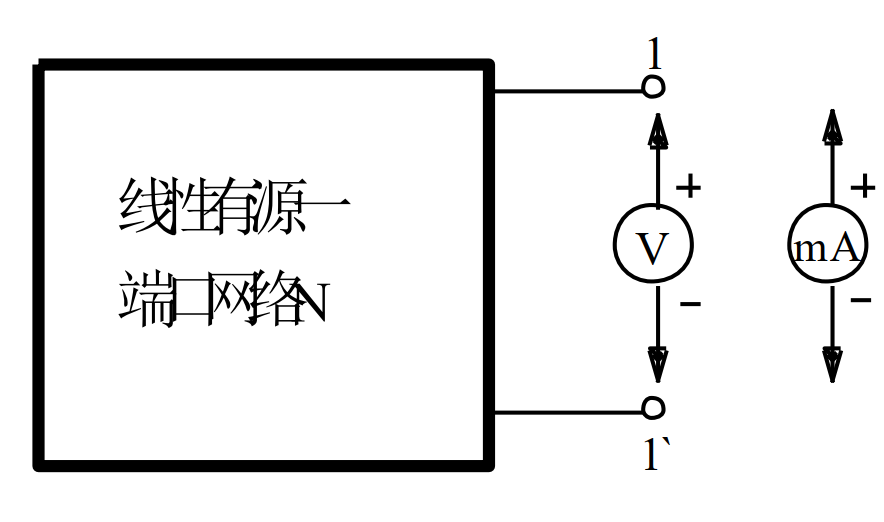
\includegraphics[width=0.4\linewidth]{开路电压.png}
			\caption{开路电压、短路电路法电路图}
			\label{}
		  \end{figure}
		 $\mathrm{U=3.93V~,~I=19.609mA}$
		  \item 间接测量法(补偿法)
		 \begin{figure}[H]
			\centering
			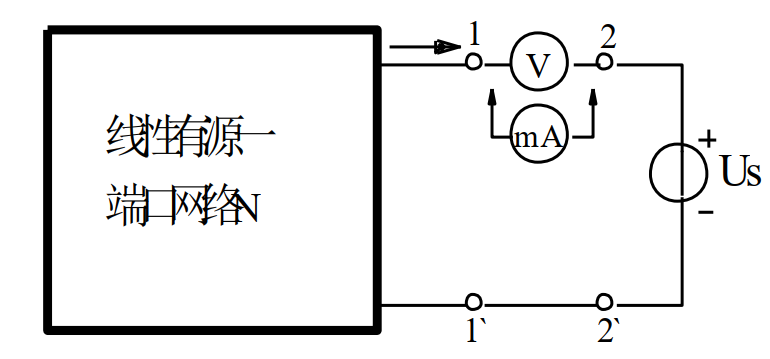
\includegraphics[width=0.4\linewidth]{电压零.png}
			\caption{间接测量法电路图}
			\label{}
		 \end{figure}
		 \begin{enumerate}
	     
		 \item 电压零示法\\
		 $\text{最初设定外加电压为 3.9V、0.1A   电压(电压表零示数结果):2.665mV }$\\
		 最终调节外加电压为$\text{U=3.93V}$
		 
		 \item 电路零示法\\
		 $\text{ 最初设定外加电压为 3.9V、0.1A  电流(电流表零示数结果):0.112mA }$\\
		 最终调节外加电压为$\text{U=3.93V}$
		 
		 \end{enumerate}	
		 
		 \item 测量等效电阻
		 
	    
		
	\end{enumerate}	


	
	% ---
	
	% 原始数据
	\clearpage
	\subsection{原始数据记录}
	实验记录本上的原始数据见%\cref{}(签字)。
	
	实验台桌面整理见%\textbf{附件}部分(\cref{})。
	
	其它原始数据见%\cref{}。
	% ---
	
	% 问题记录
	\subsection{实验过程遇到问题及解决办法}
	\begin{enumerate}
		\item 
	\end{enumerate}
	% ---
	
	
	
	% 分析与讨论	
	\clearpage
	
	% 顶栏
	\begin{table}
		\renewcommand\arraystretch{1.7}
		\begin{tabularx}{\textwidth}{|X|X|X|X|}
			\hline
			专业:& 物理学 &年级:& 2022级\\
			\hline
			姓名: &  & 学号:& \\
			\hline
			日期:&  & 评分: &\\
			\hline
		\end{tabularx}
	\end{table}
	% ---
	
	% 小标题
	\section{ETX 实验名称××× \quad\heiti 分析与讨论}
	% ---
	
	% 数据处理
	\subsection{实验数据分析}
	
	%
	\subsubsection{}
	\begin{enumerate}
		\item 
	\end{enumerate}
	
	%
	\subsubsection{}
	\begin{enumerate}
		\item 
	\end{enumerate}
	
	%
	\subsubsection{}
	
	% ---
	
	% 实验后思考题
	\subsection{实验后思考题}
	
	%思考题1
	\begin{question}
		
	\end{question}
	
	% 思考题2
	\begin{question}
		
	\end{question}
	
	% 思考题3
	\begin{question}
		
	\end{question}
	
	% ---
	
	
	% 结语部分
	\clearpage
	
	% 小标题
	\section{ETX 实验名称××× \quad\heiti 结语}
	% ---
	
	% 总结、杂谈与致谢
	\subsection{实验心得和体会、意见建议等}
	\begin{enumerate}
		\item 
	\end{enumerate}
	% ---
	

	% 附件
	\subsection{附件及实验相关的软硬件资料等}
	试验台桌面整理如%\cref{}所示。
	
	实验报告个人签名如

	% ---
	
	
\end{document}